%%%%%%%%%%%%%%%%%%%%%%%%%%%%%%%%%%%%%%%%%
% University/School Laboratory Report
% LaTeX Template
% Version 3.1 (25/3/14)
%
% This template has been downloaded from:
% http://www.LaTeXTemplates.com
%
% Original author:
% Linux and Unix Users Group at Virginia Tech Wiki
% (https://vtluug.org/wiki/Example_LaTeX_chem_lab_report)
%
% License:
% CC BY-NC-SA 3.0 (http://creativecommons.org/licenses/by-nc-sa/3.0/)
%
%%%%%%%%%%%%%%%%%%%%%%%%%%%%%%%%%%%%%%%%%

%----------------------------------------------------------------------------------------
%	PACKAGES AND DOCUMENT CONFIGURATIONS
%----------------------------------------------------------------------------------------

\documentclass{article}
\usepackage[a4paper, total={7in, 9in}]{geometry}
\usepackage[version=3]{mhchem} % Package for chemical equation typesetting
\usepackage{siunitx} % Provides the \SI{}{} and \si{} command for typesetting SI units
\usepackage{graphicx} % Required for the inclusion of images
\usepackage{natbib} % Required to change bibliography style to APA
\usepackage{amsmath} % Required for some math elements
\usepackage{booktabs}
\usepackage{physics}
\usepackage{minted}
\usepackage{subcaption}


\setlength\parindent{0pt} % Removes all indentation from paragraphs
\DeclareSIUnit\neutron{n}

  % \renewcommand{\labelenumi}{\alph{enumi}.} % Make numbering in the enumerate environment by letter rather than number (e.g. section 6)

%\usepackage{times} % Uncomment to use the Times New Roman font

%----------------------------------------------------------------------------------------
%	DOCUMENT INFORMATION
%----------------------------------------------------------------------------------------

\title{Practical Monte Carlo using MCNP \\ Assessed exercises} % Title

\author{Angus \textsc{Hollands}} % Author name

\date{\today} % Date for the report

\begin{document}

\maketitle % Insert the title, author and date


% If you wish to include an abstract, uncomment the lines below
\begin{abstract}
  A Monte Carlo simulation was performed for \num{20000} source histories, to model the light water moderated neutron fluence from a fission neutron source through the sides of a stainless steel bucket. The resulting fluence histograms were recorded, plotted against energy, and the statistical reliablity of the data evaluated. One set of tally results were not found to be reliable after failing the tally fluctation chart (TFC) Figure of Merit (FoM) slope test. The simulation was subsequently repeated for \num{200000} source histories, and the corresonding statistical reliablity of the data re\textendash evaluated. It was found that simulating \num{200000} source histories was sufficient for both flux tallies to pass the ten TFC tests, indicating result reliability.

  A second Monte Carlo model was designed to investigate the reactivity coefficient $k_{\text{eff}}$ of a simplified four cylinder enriched uranium reactor system. Several simulations were performed for two enrichments (\SI{20}{\percent}\ce{^{235}U}, \SI{25}{\percent}\ce{^{235}U}) and two moderators (graphite, light water). The reactivity coefficients were found (in product order) to be \num{0.84484\pm0.000794}, \num{0.93239 \pm 0.00074}, \num{0.89379\pm 0.00080}, and \num{1.00662 \pm 0.00077}, respectively.
\end{abstract}

\section{Introduction}
In this report, a preliminary exercise exploring process of specifying MCNP geometry was completed. Several simple geometries were defined, using the various non\textendash macrobody primitives available. The surface tallying feature was used to obtain two energy dependent histograms describing the neutron fluence distribution incident upon surfaces within a problem geometry, and an investigation was performed into the condititions under which these tallies are invalidated. For these investigations, a neutron source was configured using the Watt Fission prompt neutron spectrum for \ce{^{235}U}, with parameters referenced from the MCNP user manual.

In a subsequent exercise, a method of estimating the reactivity coefficient of a system using the KCODE card was used to investigate the effect of varying the moderator material and fuel enrichment. The definition of a concrete floor serves a secondary purpose to shielding; to reflect a fraction of the neutrons back into the vessel. Four enriched uranium cylinders were used as fissile material for the KCODE algorithm, to serve as neutron sources for the next fission cycle. The primary neutron sites were provided as initialisation parameters for the algorithm, using the KSRC card.

\section{Method}
  \subsection{Exercise 1}
    \label{sec:ex_1}
    An MCNP input file was written to design the simulation model (see Appendix~\ref{lst:ex_1}). A stainless steel vessel (of  density \SI{7.92}{\gram\per\cm^3}) with internal base \SI{10}{\cm} by \SI{20}{\cm}, wall thickness \SI{2}{\mm}, and external height \SI{20}{\cm} was modelled as the intersection between two cuboids, centered about the z axis with the lower floor placed at $z=0$.
    \begin{figure}[htb]
      \centering
      \includegraphics[width=0.3\textwidth]{cuboid.png}
      \caption{2D XZ plot of Exercise 1 geometry.}
      \label{fig:ex_1_geometry}
    \end{figure}
    The moderator was defined as the intersection between the internal cuboid and an infinite planar surface of normal $\mqty(0 & 0 & -1)$ at $\mqty(0 & 0 & 19.0)$. Two void regions were then defined, one for the volume outside of the outer cuboid, and the other for the region between the moderator surface and the plane bounding the outer cuboid ceiling.
    All cells were defined with a neutron importance of $1$, apart from the outer void region, and their materials appropriately defined in the DATA section.
    All cells were assigned a material with the appropriate atomic / weight composition, and assigned with the correct weight density. The moderator was assiged the light water low energy cross section library \textit{lwtr.01[t]}.
    Two surface neutron flux tally cards were defined, using a common set of energy bins, with upper bin edges defined along the loglinear interval between \SI{1e-9}{\MeV} and \SI{10}{\MeV}. One tally recorded the flux through the two short external sides of the vessel, and the other recorded the corresponding flux through the two larger sides.
    A thermal neutron source with an energy distribution given by the Watt Fission spectrum for \ce{^{235}U} (see Fig~\ref{fig:watt_fission}), with parameters $a=0.988$, $b=2.249$, was placed at $\mqty(0 & 0 & 2.2)$, and the simulation performed for \num{20000} neutrons (MODE N) source histories. A secondary simulation was performed with an increased number of source histories of \num{200000}.
    \begin{figure}[htb]
      \centering
      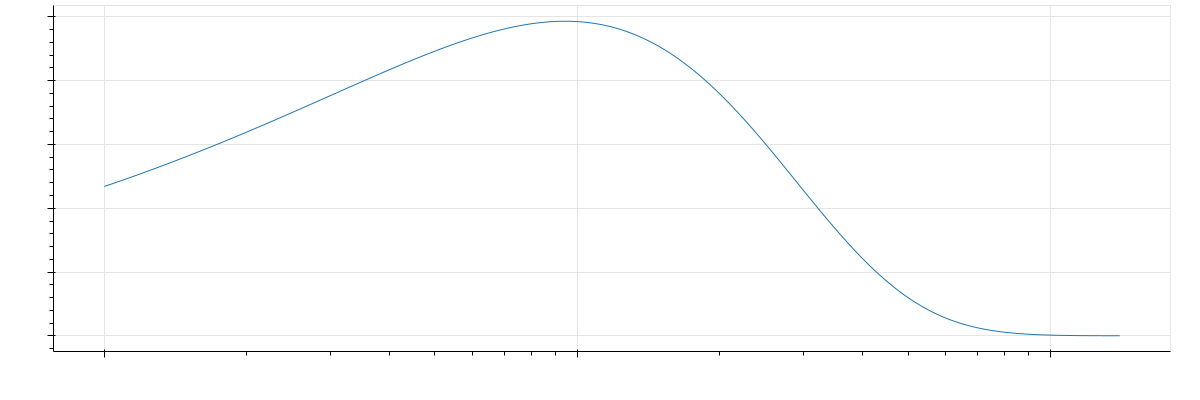
\includegraphics[width=\textwidth]{watt_spectrum_235_u.png}
      \caption{Watt Fission spectrum for prompt neutrons (\ce{^{235}U}).} % TODO chite https://ac.els-cdn.com/S1875389215001236/1-s2.0-S1875389215001236-main.pdf?_tid=946afe26-9e8b-4e65-afa5-899d0c8d8665&acdnat=1523017641_ed02eb00bf5004212d9cca7c0116a978
      \label{fig:watt_fission}
    \end{figure}

  \subsection{Exercise 3}
    The geometry described in Section~\ref{sec:ex_1} was modified such that the internal base measured \SI{100}{\cm} by \SI{100}{\cm}, with an external height of \SI{60}{\cm}.
    A concrete floor was defined, of thickness \SI{304.8}{\cm}, and a lateral radius of \SI{500}{\cm}. These two parameters were not defined in the exercise requirements; the former was taken from relevant literature, and the latter chosen to be significantly greater than the floor thickness. % TODO explain why
    The moderator volume was resized to satisfy the original wall thickness constraints, and the surface moved to \SI{2}{\cm} from the ceiling of the vessel. For each simulation, the appropriate moderator material was defined (for graphite / water), and the corresponding low energy cross section library referenced (\textit{lwtr.01[t]} / \textit{grph.01[t]})
    Four enriched uranium cylindrical sources, of radius \SI{7.5}{\cm} and height \SI{25}{\cm}, were placed within the moderator cell. The fuel material card was defined for a by\textendash weight enrichment which was varied across several of the simulations.
    The KCODE Monte Carlo eigenvalue algorithm was used to determine the reactivity coefficient $k_{\text{eff}}$ of the system. The KSRC card was used to distribute 1000 starting neutrons across the centroids of the uranium cylinders. The KCODE algorithm was configured for a warm up of 200 cycles, with an initial reactivity estimate of 1.0 (critical), and run for 1000 active cycles. As with Section~\ref{sec:ex_1}, only the outermost void cell was given a zero neutron importance, with the remaining cell neutron importances set to unity.
    \begin{figure}[htb]
      \centering
      \includegraphics[width=0.3\textwidth]{criticality.png}
      \caption{2D XZ plot of Exercise 3.d. (Graphite) geometry.}
      \label{fig:ex_3_d_2_geometry}
    \end{figure}

\section{Results}
  \subsection{Exercise 1}
    \subsubsection{Initial Simulation}
      \begin{figure}[htb]
        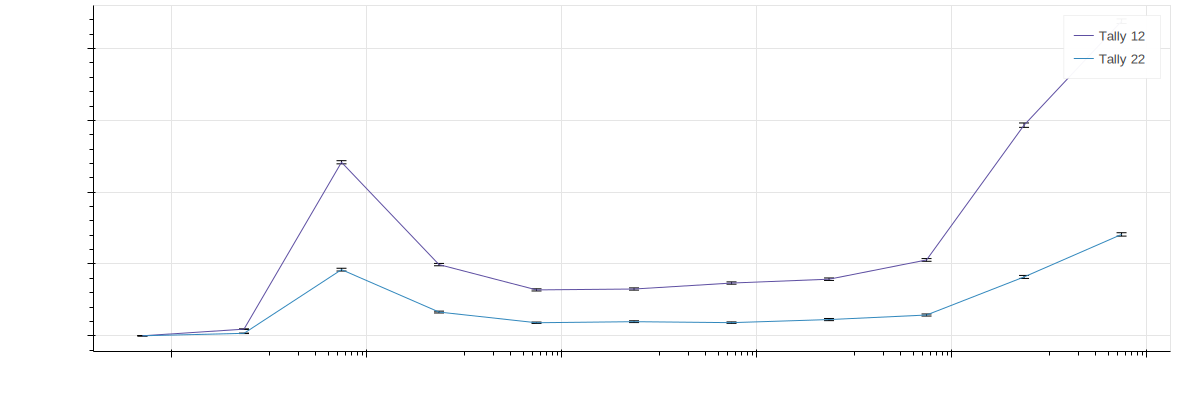
\includegraphics[width=\textwidth]{tallies.png}
        \caption{Fluence tallies for external surfaces of container, for \num{20000} histories. Tally 12 corresponds to the fluence across the shorter sides of the container, 22 the longer sides.}
        \label{fig:tallies_20000}
      \end{figure}

%TODO table
    The tallies are defined as follows:
    \begin{itemize}
      \item Tally 12: The short sides of characteristic length \SI{10}{\cm}
      \item Tally 22: The long sides of characteristic length \SI{20}{\cm}
    \end{itemize}

    For the tallies, MCNP reported that the tallies passed most of the 10 statistical tests for the tally fluctuation chart, which are defined as
    \begin{enumerate}
      \item Mean is randomly distributed
      \item Relative error ideally less than $0.10$
      \item Relative error decreases over time
      \item Decrease rate of relative error follows $\frac{1}{\sqrt{\text{nps}}}$
      \item Variance of variance ideally less than $0.10$
      \item Variance of variance decreases over time
      \item Decrease rate of variance of variance follows $\frac{1}{\sqrt{\text{nps}}}$
      \item Figure of Merit (FoM) is roughly constant
      \item FoM is randomly distributed
      \item Slope of the FoM pdf is greater than $3.0$
    \end{enumerate}
    The first and last tallies passed all ten tests, whilst Tally 22 failed the final FoM slope PDF test. In addition, all tallies had at least one bin with large relative error ($>0.1$).

    The total fluences across each pair of surfaces were as follows
    \begin{itemize}
      \item Long sides (Tally 12): \SI{7.70884\pm0.093277e-4}{\neutron\per\cm^2}
      \item Short sides (Tally 34): \SI{2.53400 \pm 0.082862e-4}{\neutron\per\cm^2}
    \end{itemize}
    \begin{figure}[htb]
      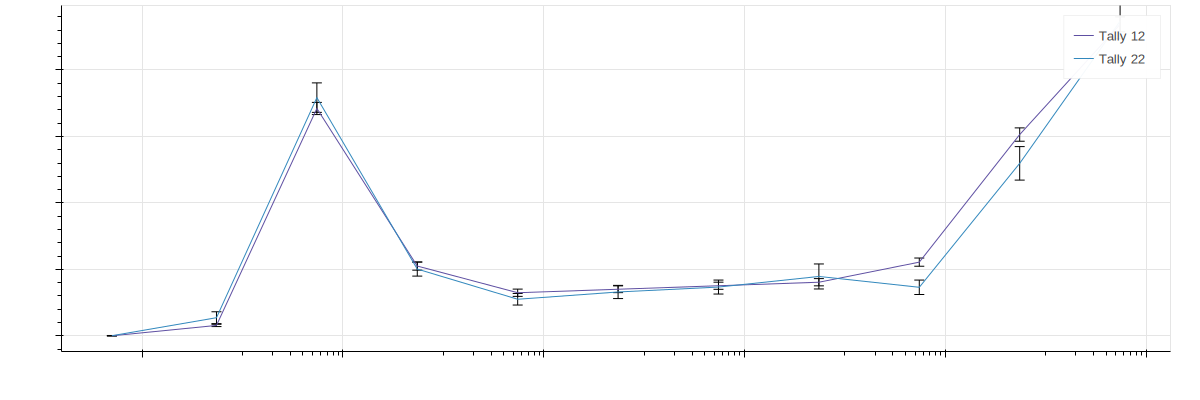
\includegraphics[width=\textwidth]{tallies_norm.png}
      \caption{Area normalised fluence tallies for external surfaces of container, for \num{20000} histories. Tally 12 corresponds to the fluence across the shorter sides of the container, 22 the longer sides.}
      \label{fig:tallies_20000_norm}
    \end{figure}

    \subsubsection{Flux}
    For a source of $10^{10}$ neutrons per second, the corresponding fluxes would be \SI{7.70884\pm 0.093277e+6}{\neutron\per\cm^2\per\second} and \SI{2.53400 \pm 0.082862e+6}{\neutron\per\cm^2\per\second} respectively.

    \subsubsection{Increasing Number of Histories}
      By increasing the particle histories limit to $200000$, the standard uncertainty upon the tally amplitudes diminishes, approximately $\frac{1}{2}$ as expected. The bin amplitude for Tally 22 corresponding to $(\num{1e-8} < x <\num{1e-9})$ did not lie within the uncertainty permitted by its previous value. However, this tally did not pass all statistical tests for $20000$ to allow such a constraint in the first place, and so was to be expected. By increasing the number of particle histories to the new limit, all statistical tests were subsequently passed. Furthermore, the difference in neutron energy distribution between the two tallies became more apparent; in particular, in the higher energy regime the two distributions diverged most significantly, with the narrower surfaces (further from the source) showing greater attenuation at higher energies.
      The recorded fluences were as follows:
      \begin{itemize}
          \item Long sides (Tally 12): \SI{7.65531\pm 0.029856e-4}{\neutron\per\cm^2}
          \item Short sides (Tally 34): \SI{2.5150\pm 0.025402e-4}{\neutron\per\cm^2}
      \end{itemize}

  \subsection{Exercise 3}
    \begin{table}[]
    \centering
    \caption{Reactivity coefficient for various simulated scenarios.}
    \label{table:reactivities}
    \begin{tabular}{@{}ccc@{}}
    \toprule
    Moderator & Enrichment & $k_{\text{eff}}$      \\ \midrule
    Light water        & \SI{20}{\percent} & \num{0.84484\pm0.000794}   \\
    Graphite           & \SI{20}{\percent} & \num{0.93239 \pm 0.00074} \\
    Light water        & \SI{25}{\percent} & \num{0.89379\pm 0.00080}  \\
    Graphite           & \SI{25}{\percent} & \num{1.00662 \pm 0.00077} \\ \bottomrule
    \end{tabular}
    \end{table}


\section{Analysis}
  \subsection{Exercise 1}
    The final FoM slope test evaluates whether the central limit theorem has been satisfied; that is, both the first and second moments of the PDF exist (and are therefore finite). The second moment $\int_{\infty}^{\infty}{x^2f(x)\operatorname{dx}}$ is observed to exist when $f(x)$ decreases faster than $\frac{1}{x^3}$, and hence the final test evaluates this condition. Consequently, in failing this test for the initial simulation, it cannot be concluded that Tally 22 is reliable.

    The significant difference between the total fluences for the two tallies can be explained by both the variation in solid angle between the two surfaces (each surface is sufficiently large relative to the distance to the source, that the incident flux varies along the surface), and the difference in neutron absorption along the axes of the detector. The neutron absorption probability through a medium is given by the Beer Lambert law, and is exponential in the distance travelled.
    The normalised (by area) neutron energy distributions are approximately equal, and what variation there exists between the two tallies lies predominantly within the uncertainty on the recorded values. However, there are several points, particularly in the higher energy regime whose standard errors do not account for the observed deviation. In these cases, the nonlinear attenuation function, which depends upon neutron energy, leads to a distortion of the tallied energy spectrum.

  \subsection{Exercise 3}
    \subsubsection{Graphite Moderator}
    When replacing the moderator material with graphite, the effective criticality of the system was observed to increase. The criticality of a reactor depends upon the number of neutrons which are thermalised (by the moderator) and lead to thermal fission in the fuel. In transitioning the moderator material from light water to graphite, the mean logarithmic energy decrement of the moderator $\xi$ decreases (lesser energy loss per collision), such that the average number of collisions required to thermalise a fast neutron increases by a factor $\frac{\xi_{H_2O}}{\xi_{C}}=5.8\,.$
    However, the scattering to capture ratio of graphite is far higher than that of light water ($1500$ vs $77.17$), and thus its effective "moderating ratio" $\frac{\xi\sigma_{s}}{\sigma_{a}}$ is greater. This result was observed in the predicted reactivity coefficients for the two systems. In the case of the graphite moderator, the reactivity coefficient was greater (closer to criticality) than that of the light water.
    For both moderators, the application of the Shapiro\textendash Wilke (W) test for normality indicated that the results are normally distributed with a \SI{95}{\percent} confidence interval for all of the reactivity estimators.

    \subsubsection{Increasing Enrichment}
    After increasing the enrichment of the uranium cylinders, the reactivity coefficient of both modelled systems was observed to increase. Similarly to the previous configuration, the predicted coefficient for the graphite moderator remained greater than that of the light water.
    As for the previous scenario, the application of the Shapiro\textendash Wilke (W) test for normality indicated that the results are normally distributed with a \SI{95}{\percent} confidence interval for all of the reactivity estimators.

    \begin{figure}
      \includegraphics[width=\textwidth]{cross_sections.png}
      \caption{Fission cross sections of \ce{^{238}U} and \ce{^{235}U}}
      \label{fig:cross_sections}
    \end{figure}

    The observed increase in reactivity derives from the increased effective fission cross section of the fuel that follows fuel enrichment (see \ref{fig:cross_sections}). $^{235}\text{U}$ has a greater fission cross section than $^{238}\text{U}$, and thus increasing the ratio of $^{235}\text{U}$ to $^{238}\text{U}$ in the fuel serves to increase the fission probability, moving the system towards criticality (see $Fig~$).

\section{Conclusions}
  In completing the two exercises, several important observations were made concerning the various MCNP features which may be used to ensure valid results, and identify problematic cases (such as undersampled paths). The final exercise shows explicitly the importance of selecting the correct fuel enrichment, and moderator material, to avoid a reactor becoming supercritical on prompt neutrons alone.


\section{Appendix}
    \captionof{listing}{Exercise 1. MCNP input file.\label{lst:ex_1}}
    \inputminted{lexer.py -x}{mcnp/1.ip}

    \captionof{listing}{Exercise 3.d. (Graphite) MCNP input file.\label{lst:ex_3_d_2}}
    \inputminted{lexer.py -x}{mcnp/3.d.2.ip}
\end{document}
